\documentclass{beamer}

\usepackage[T2A]{fontenc}
\usepackage[utf8]{inputenc}
\usepackage[english,russian]{babel}
\input{settings.tex}


\title{Дуальность, Чувствительность, KKT}
\subtitle{Вычислительный интеллект, Лекция  13}
\author{Сергей Савин}
\centering
\date{\mydate}



\begin{document}
\maketitle


%\begin{frame}{Content}
%
%\begin{itemize}
%\item Lagrange dual function
%\item Duality gap, strong and weak duality
%\item KKT conditions
%\item Sensitivity
%\end{itemize}
%
%\end{frame}





\begin{frame}{Лагранжиан}
	\begin{flushleft}
		
		Рассмотрим задачу оптимизации:
		
		\begin{equation}
			\begin{aligned}
				& \underset{\bo{x}}{\text{minimize}}
				& & f_0(\bo{x}), \\
				& \text{subject to}
				& & \begin{cases}
					f_i(\bo{x}) \leq 0, \\
					h_j(\bo{x}) = 0.
				\end{cases}
			\end{aligned}
		\end{equation}
		
		Её \emph{лагранжиан} задаётся как:
		
		\begin{equation}
			L(\bo{x}, \lambda_i, \nu_j) = 
			f_0(\bo{x}) + 
			\sum\limits_i \lambda_i f_i(\bo{x}) +
			\sum\limits_j \nu_j h_j(\bo{x})
		\end{equation}
		%
		где $\lambda_i \geq 0$ и $\nu_j$ — множители Лагранжа; их также иногда называют \emph{двойственными переменными}.
		
	\end{flushleft}
\end{frame}

\begin{frame}{Условия ККТ}
	\begin{flushleft}
		
		Условия Каруша — Куна — Таккера (KKT) подтверждают оптимальность задачи оптимизации:
		
		\begin{equation}
			\begin{aligned}
				& \underset{\bo{x}}{\text{minimize}}
				& & f_0(\bo{x}), \\
				& \text{subject to}
				& & \begin{cases}
					f_i(\bo{x}) \leq 0, \\
					h_j(\bo{x}) = 0.
				\end{cases}
			\end{aligned}
		\end{equation}
		
		\begin{enumerate}
			\item Прямая допустимость: $f_i(\bo{x}) \leq 0$ и $h_j(\bo{x}) = 0$.
			
			\item Двойственная допустимость: $\lambda_i \geq 0$.
			
			\item Дополняющая нежёсткость: $\lambda_i f_i(\bo{x}) = 0$.
			
			\item Стационарность лагранжиана: $\frac{\partial}{\partial \bo{x}} 
			\left ( f_0(\bo{x}) + 
			\sum\limits_i \lambda_i f_i(\bo{x}) +
			\sum\limits_j \nu_j h_j(\bo{x}) \right ) = 0$.
		\end{enumerate}
		
	\end{flushleft}
\end{frame}

\begin{frame}{Двойственная функция Лагранжа}
	\begin{flushleft}
		
		Для \emph{лагранжиана} $L(\bo{x}, \lambda_i, \nu_j) = 
		f_0(\bo{x}) + 
		\sum\limits_i \lambda_i f_i(\bo{x}) +
		\sum\limits_j \nu_j h_j(\bo{x})$, соответствующая 
		\emph{двойственная функция Лагранжа} задаётся как:
		
		\begin{equation}
			g(\lambda_i, \nu_j)  = \underset{\bo{x}}{\text{inf}}
			\ L(\bo{x}, \lambda_i, \nu_j).
		\end{equation}
		
		Двойственная функция Лагранжа \textbf{всегда вогнута}. Если $p^*$ — оптимальное значение целевой функции исходной задачи, то $g(\lambda_i, \nu_j)$ даёт \emph{нижнюю границу} её возможных значений:
		
		\begin{equation}
			g(\lambda_i, \nu_j)  \leq L(\bo{x}^*, \lambda_i, \nu_j)  \leq f_0(\bo{x}^*)
		\end{equation}
		
		Фактически, подстановка любых $\nu_j$ и $\lambda_i \geq 0$ даёт нам допустимую нижнюю границу стоимости. Максимум $g(\lambda_i, \nu_j)$ по области, заданной условием $\lambda_i \geq 0$, даёт нам оптимальную (наибольшую) нижнюю границу задачи, обозначаемую как $g^*$. 
		
	\end{flushleft}
\end{frame}

\begin{frame}{Двойственный разрыв, сильная и слабая двойственность}
	\begin{flushleft}
		
		Если $p^*$ — оптимальное значение целевой функции исходной задачи, а $g^*$ — оптимальная нижняя граница задачи, то $p^* - g^*$ называется оптимальным \emph{двойственным разрывом}.
		
		\bigskip
		
		Если оптимальный двойственный разрыв равен нулю, говорят, что задача обладает \emph{сильной двойственностью}. Если оптимальный двойственный разрыв больше нуля, говорят, что задача обладает \emph{слабой двойственностью}.
		
	\end{flushleft}
\end{frame}
\begin{frame}{Двойственная функция Лагранжа для квадратичной задачи, 1}
	\begin{flushleft}
		
		Рассмотрим следующую квадратичную задачу оптимизации (QP):
		
		\begin{equation}
			\begin{aligned}
				& \underset{\bo{x}}{\text{minimize}}
				& & \bo{x}^\top \bo{H} \bo{x}, \\
				& \text{subject to}
				& & \bo{A}\bo{x} \leq \bo{b}.
			\end{aligned}
		\end{equation}
		%
		Её лагранжиан:
		%
		\begin{equation}
			L(\bo{x}, \lambda) = \bo{x}^\top \bo{H} \bo{x} + \lambda^\top (\bo{A}\bo{x} - \bo{b})
		\end{equation}
		
		Чтобы минимизировать лагранжиан по $\bo{x}$, найдём градиент и приравняем его к нулю:
		%
		\begin{equation}
			\frac{\partial L(\bo{x}, \lambda)}{\partial \bo{x}} = 2\bo{x}^\top \bo{H} + \lambda^\top \bo{A} = 0
		\end{equation}
		
		Отсюда можно выразить $\bo{x}$ как функцию $\lambda$:
		%
		\begin{equation}
			\bo{x} = -0.5\bo{H}^{-1}\bo{A}^\top \lambda
		\end{equation}
		
	\end{flushleft}
\end{frame}

\begin{frame}{Двойственная функция Лагранжа для квадратичной задачи, 2}
	\begin{flushleft}
		
		Зная, что $\bo{x} = -0.5\bo{H}^{-1}\bo{A}^\top \lambda$, можно вычислить $g(\lambda)$, подставив найденный $\bo{x}$ в лагранжиан:
		%
		\begin{equation}
			g(\lambda) = \frac{1}{4} \lambda^\top \bo{A}\bo{H}^{-1}\bo{H}\bo{H}^{-1}\bo{A}^\top\lambda - \frac{1}{2} \lambda^\top \bo{A}\bo{H}^{-1}\bo{A}^\top \lambda - \lambda^\top\bo{b}
		\end{equation}
		%
		\begin{equation}
			g(\lambda) = -\frac{1}{4} \lambda^\top \bo{A}\bo{H}^{-1}\bo{A}^\top\lambda - \lambda^\top\bo{b}
		\end{equation}
		
		Чтобы найти оптимальную нижнюю границу, решим следующую задачу:
		%
		\begin{equation}
			\begin{aligned}
				& \underset{\lambda}{\text{maximize}}
				& & -\frac{1}{4} \lambda^\top \bo{A}\bo{H}^{-1}\bo{A}^\top\lambda - \lambda^\top\bo{b}, \\
				& \text{subject to}
				& & \lambda \geq 0.
			\end{aligned}
		\end{equation}
		
		Решение этой задачи является решением исходной задачи.
		
	\end{flushleft}
\end{frame}

\begin{frame}{Чувствительность}
	\begin{flushleft}
		
		Рассмотрим параметрическую задачу оптимизации
		\begin{equation}
			\begin{aligned}
				\min_{x} \quad & f(x,u) \\
				\text{s.t.} \quad & g(x,u) \leq 0,
			\end{aligned}
		\end{equation}
		где $x \in \mathbb{R}^n$ — переменная решения, а $u \in \mathbb{R}^p$ — параметр.
		
		Пусть $x^*(u)$ обозначает оптимальное решение. \textbf{Функция значения} определяется как
		\begin{equation}
			v(u) := f(x^*(u), u).
		\end{equation}
		
		
		Анализ чувствительности изучает, как оптимальное значение изменяется при возмущениях параметра $u$, то есть
		\begin{equation}
			\text{чувствительность по } u = \frac{dv}{du}.
		\end{equation}
		
	\end{flushleft}
\end{frame}

\begin{frame}{Теорема об огибающей, 1}
	\begin{flushleft}
		
		Определим лагранжиан:
		\begin{equation}
			\mathcal{L}(x,\lambda,u) = f(x,u) + \lambda^\top g(x,u).
		\end{equation}
		
		Тогда производная функции значения равна
		\begin{equation*}
			\boxed{
				\frac{dv}{du}
				=
				\frac{\partial \mathcal{L}(u)}{\partial u}.}
		\end{equation*}
		
		По определению,
		\begin{equation}
			v(u) = f(x^*(u), u).
		\end{equation}
		Применяя правило цепочки,
		\begin{equation}
			\frac{dv}{du}
			=
			\frac{\partial f}{\partial x} \frac{dx^*}{du}
			+
			\frac{\partial f}{\partial u}.
		\end{equation}
		
	\end{flushleft}
\end{frame}

\begin{frame}{Теорема об огибающей, 2}
	\begin{flushleft}
		
		\begin{equation}
			\frac{dv}{du}
			=
			\textcolor{mygreen}{\frac{\partial f}{\partial x}} \frac{dx^*}{du}
			+
			\frac{\partial f}{\partial u}.
		\end{equation}
		
		В точке оптимума условие стационарности даёт
		\begin{equation}
			\textcolor{mygreen}{\frac{\partial f}{\partial x}} 
			+
			\left( \frac{\partial g}{\partial x} \right)^\top \lambda^*
			=
			0. 
			\quad \rightarrow \quad
			%
			\textcolor{mygreen}{\frac{\partial f}{\partial x}} 
			=
			- \lambda^{*\top} \frac{\partial g}{\partial x}.
		\end{equation}
		
		Подставим в $\frac{dv}{du}$:
		\begin{equation}
			\frac{dv}{du}
			=
			- \lambda^{*\top} 
			\textcolor{myblue}{ \frac{\partial g}{\partial x} \frac{dx^*}{du}}
			+
			\frac{\partial f}{\partial u}.
		\end{equation}
		
		Для активных ограничений $g(x^*(u), u) = 0.$
		Дифференцируя,
		\begin{equation}
			\textcolor{myblue}{\frac{\partial g}{\partial x} \frac{dx^*}{du}}
			+
			\frac{\partial g}{\partial u}
			=
			0.
			\quad \rightarrow \quad
			%
			\textcolor{myblue}{\frac{\partial g}{\partial x} \frac{dx^*}{du}}
			=
			- \frac{\partial g}{\partial u}.
		\end{equation}
		
	\end{flushleft}
\end{frame}


\begin{frame}{Теорема об огибающей, 3}
	\begin{flushleft}
		
		Подставим в выражение для $\frac{dv}{du}$:
		\begin{equation}
			\frac{dv}{du}
			=
			\lambda^{*\top} \frac{\partial g}{\partial u}
			+
			\frac{\partial f}{\partial u}.
		\end{equation}
		
		
		\begin{equation}
			\boxed{
				\frac{dv}{du}
				=
				\frac{\partial f}{\partial u}
				+
				\lambda^{*\top} \frac{\partial g}{\partial u}
				=
				\frac{\partial \mathcal{L}}{\partial u}
			}
		\end{equation}
		
	\end{flushleft}
\end{frame}

\begin{frame}{Чувствительность: возмущение правой части линейного ограничения}
	\begin{flushleft}
		
		Рассмотрим задачу с возмущённым ограничением:
		
		\begin{equation*}
			\begin{aligned}
				\min_x \quad & f(x) \\
				\text{s.t.} \quad & a^\top x \le b + u.
			\end{aligned}
		\end{equation*}
		
		Определим функцию значения $v(u) = f(x^*(u))$ и лагранжиан
		\begin{equation*}
			\mathcal{L}(x,\lambda,u) = f(x) + \lambda (a^\top x - b - u).
		\end{equation*}
		
		Из теоремы об огибающей:
		\begin{equation*}
			\frac{dv}{du} = \frac{\partial \mathcal{L}}{\partial u}(x^*, \lambda^*, u) = -\lambda.
		\end{equation*}
		
		Множитель $\lambda^*$ измеряет предельную ценность ослабления ограничения. Увеличение $u$ (ослабление ограничения) уменьшает оптимальную стоимость со скоростью $\lambda^*$.
		
	\end{flushleft}
\end{frame}

\begin{frame}{Чувствительность: возмущение правой части линейного ограничения, иллюстрация}
	\begin{flushleft}
		
		\begin{figure}
			\centering
			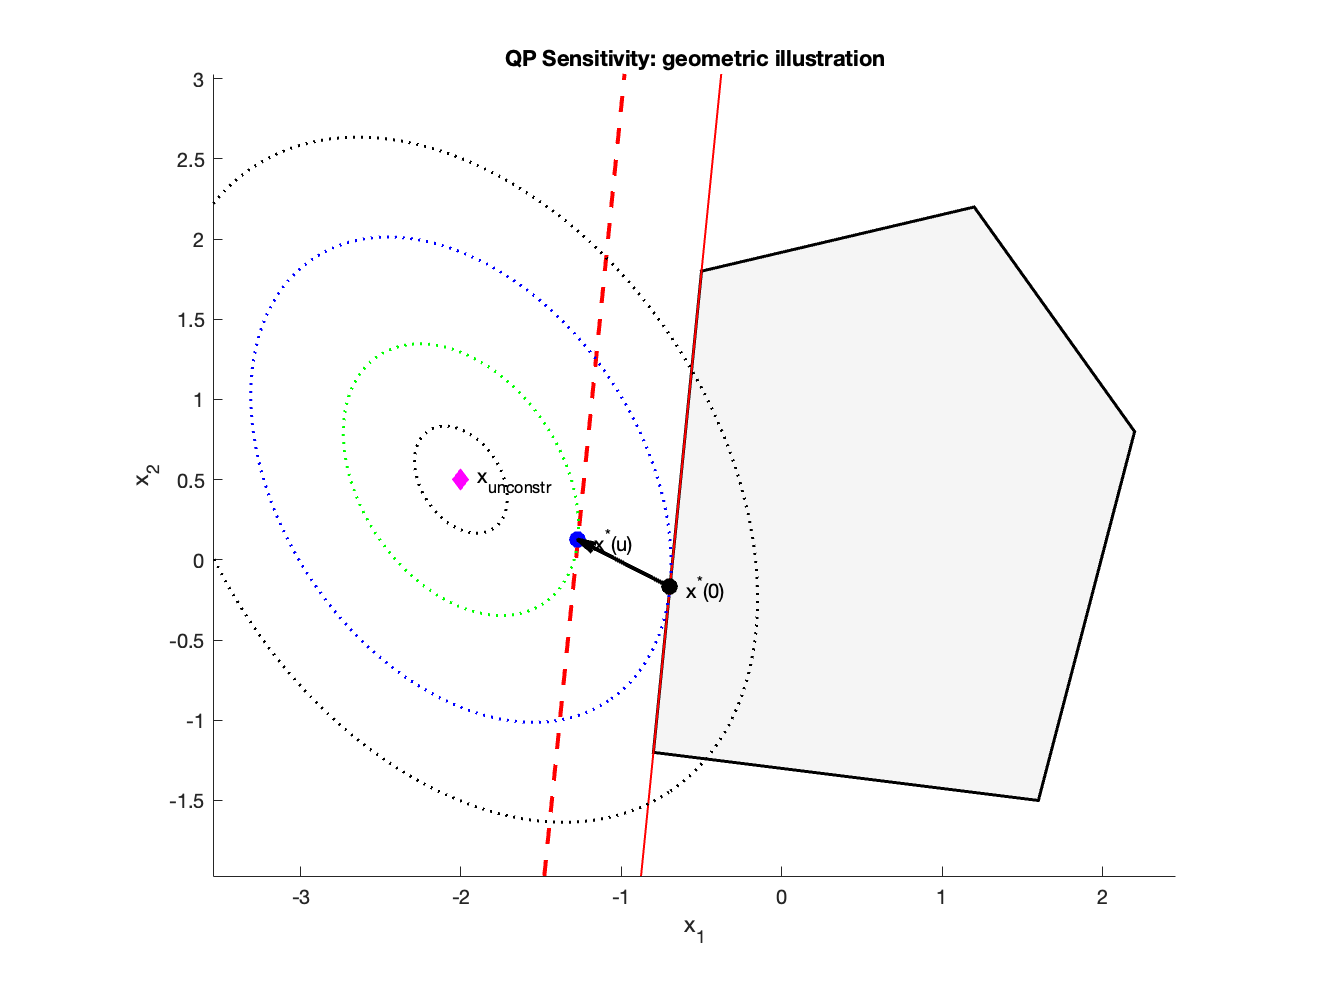
\includegraphics[width=0.9\linewidth]{illustration}
			\caption{Чувствительность по отношению к возмущению правой части линейного ограничения}
			\label{fig:illustration}
		\end{figure}
		
		
	\end{flushleft}
\end{frame}

\begin{frame}{Чувствительность: возмущение нормали ограничения}
	\begin{flushleft}
		
		Рассмотрим задачу с возмущённым направлением ограничения:
		\begin{equation*}
			\begin{aligned}
				\min_x \quad & f(x) \\
				\text{s.t.} \quad & (a + u)^\top x \le b.
			\end{aligned}
		\end{equation*}
		
		Определим функцию значения $v(u) = f(x^*(u))$ и лагранжиан
		\begin{equation*}
			\mathcal{L}(x,\lambda,u) = f(x) + \lambda \big((a+u)^\top x - b\big).
		\end{equation*}
		
		Из теоремы об огибающей:
		\begin{equation*}
			\frac{dv}{du} = \frac{\partial \mathcal{L}}{\partial u}(x^*, \lambda^*, u) = \lambda^* x^*.
		\end{equation*}
		
		
	\end{flushleft}
\end{frame}

\begin{frame}{Чувствительность: возмущение в стоимости}
	\begin{flushleft}
		
		Рассмотрим задачу с возмущённой стоимостью:
		\begin{equation*}
			\begin{aligned}
				\min_x \quad & \tfrac{1}{2} x^\top Q x + (q+u)^\top x \\
				\text{s.t.} \quad & a^\top x \le b.
			\end{aligned}
		\end{equation*}
		
		Определим функцию значения $v(u) = f(x^*(u), u)$ и лагранжиан
		\begin{equation*}
			\mathcal{L}(x,\lambda,u) = \tfrac{1}{2} x^\top Q x + (q+u)^\top x + \lambda (a^\top x - b).
		\end{equation*}
		
		Из теоремы об огибающей:
		\begin{equation*}
			\frac{dv}{du} = \frac{\partial \mathcal{L}}{\partial u}(x^*, \lambda^*, u) = x^*.
		\end{equation*}
		
		Чувствительность равна оптимальному решению: возмущение линейной стоимости изменяет оптимальное значение со скоростью, задаваемой непосредственно $x^*$.
		
	\end{flushleft}
\end{frame}





\begin{frame}{Литература}
	\begin{flushleft}
		
		\begin{itemize}
			\item \bref{https://www.stat.cmu.edu/~ryantibs/convexopt-F16/scribes/kkt-scribed.pdf}{Convex Optimization, Lecture 12: KKT conditions, Ryan Tibshirani.}
			
			\item \bref{https://people.eecs.berkeley.edu/~elghaoui/Teaching/EE227A/lecture13.pdf}{EE 227A: Convex Optimization and Applications, Lecture 13: Optimality Conditions for Convex Problems, Laurent El Ghaoui.}
			
			\item \bref{https://youtu.be/uh1Dk68cfWs?si=rHb-bFyrDeqkJo_I}{The Karush–Kuhn–Tucker (KKT) Conditions (video). Visually Explained.}
		\end{itemize}
		
		
		
		
		
		
	\end{flushleft}
\end{frame}






\myqrframe



\end{document}
